\PassOptionsToPackage{table}{xcolor}
\documentclass[portrait,final,a0paper,fontscale=0.320]{imiseposter}
\usepackage[T1]{fontenc}
\usepackage[utf8]{inputenc}
\usepackage[ngerman]{babel}% change to ngerman for a German poster
\microtypecontext{spacing=nonfrench}
% Using biblatex and biber. It's more modern but takes more than twice as long to compile in my case. ****
% If you use biblatex, you need to comment and uncomment the marked statements in the references as well.
\usepackage{csquotes}
\usepackage[style=numeric,backend=biber]{biblatex}
\addbibresource{poster.bib}
%*********************************************************************************************************
\usepackage{graphicx}
\usepackage{url}% do not use hyperref as its links are displaced with baposter because of the font scale 

\usepackage{blindtext}% remove for production

% Select Font %%%%%%%%%%%%%%%%%%%%%%%%%%%%%%%%%%%%%%%
%\usepackage{helvet} % closest to arial
\usepackage{bookman} % has some resemblance to Futura
%%%%%%%%%%%%%%%%%%%%%%%%%%%%%%%%%%%%%%%%%%%%%%%%%%%%%
\renewcommand{\familydefault}{\sfdefault}

\newcommand{\captionfont}{\footnotesize}
\usepackage[font=small,labelfont=bf]{caption}

\begin{document}

\begin{poster}% Set grid to false for final print
  {grid=true,}
  % Eye Catcher
  {
\includegraphics[height=4.5cm, width=10cm, keepaspectratio]{img/logos/wog-logo-ohne-text.pdf}} 
  % Title
  {Question Answering auf SNIK}
  % Authors
  {Hannes R. Brunsch}
  % SNIK ontology logo
  {
\includegraphics[height=9.0em]{img/logos/snik-logo.png}}

%%%%%%%%%%%%%%%%%%%%%%%%%%%%%%%%%%%%%%%%%%%%%%%%%%%%%%%%%%%%%%%%%%%%%%%%%%%%%%
\begin{posterbox}[name=background,column=0,row=0]{Hintergrund}
Some text~\cite{bb} and some more text~\cite{ob} and even more text~\cite{he}.
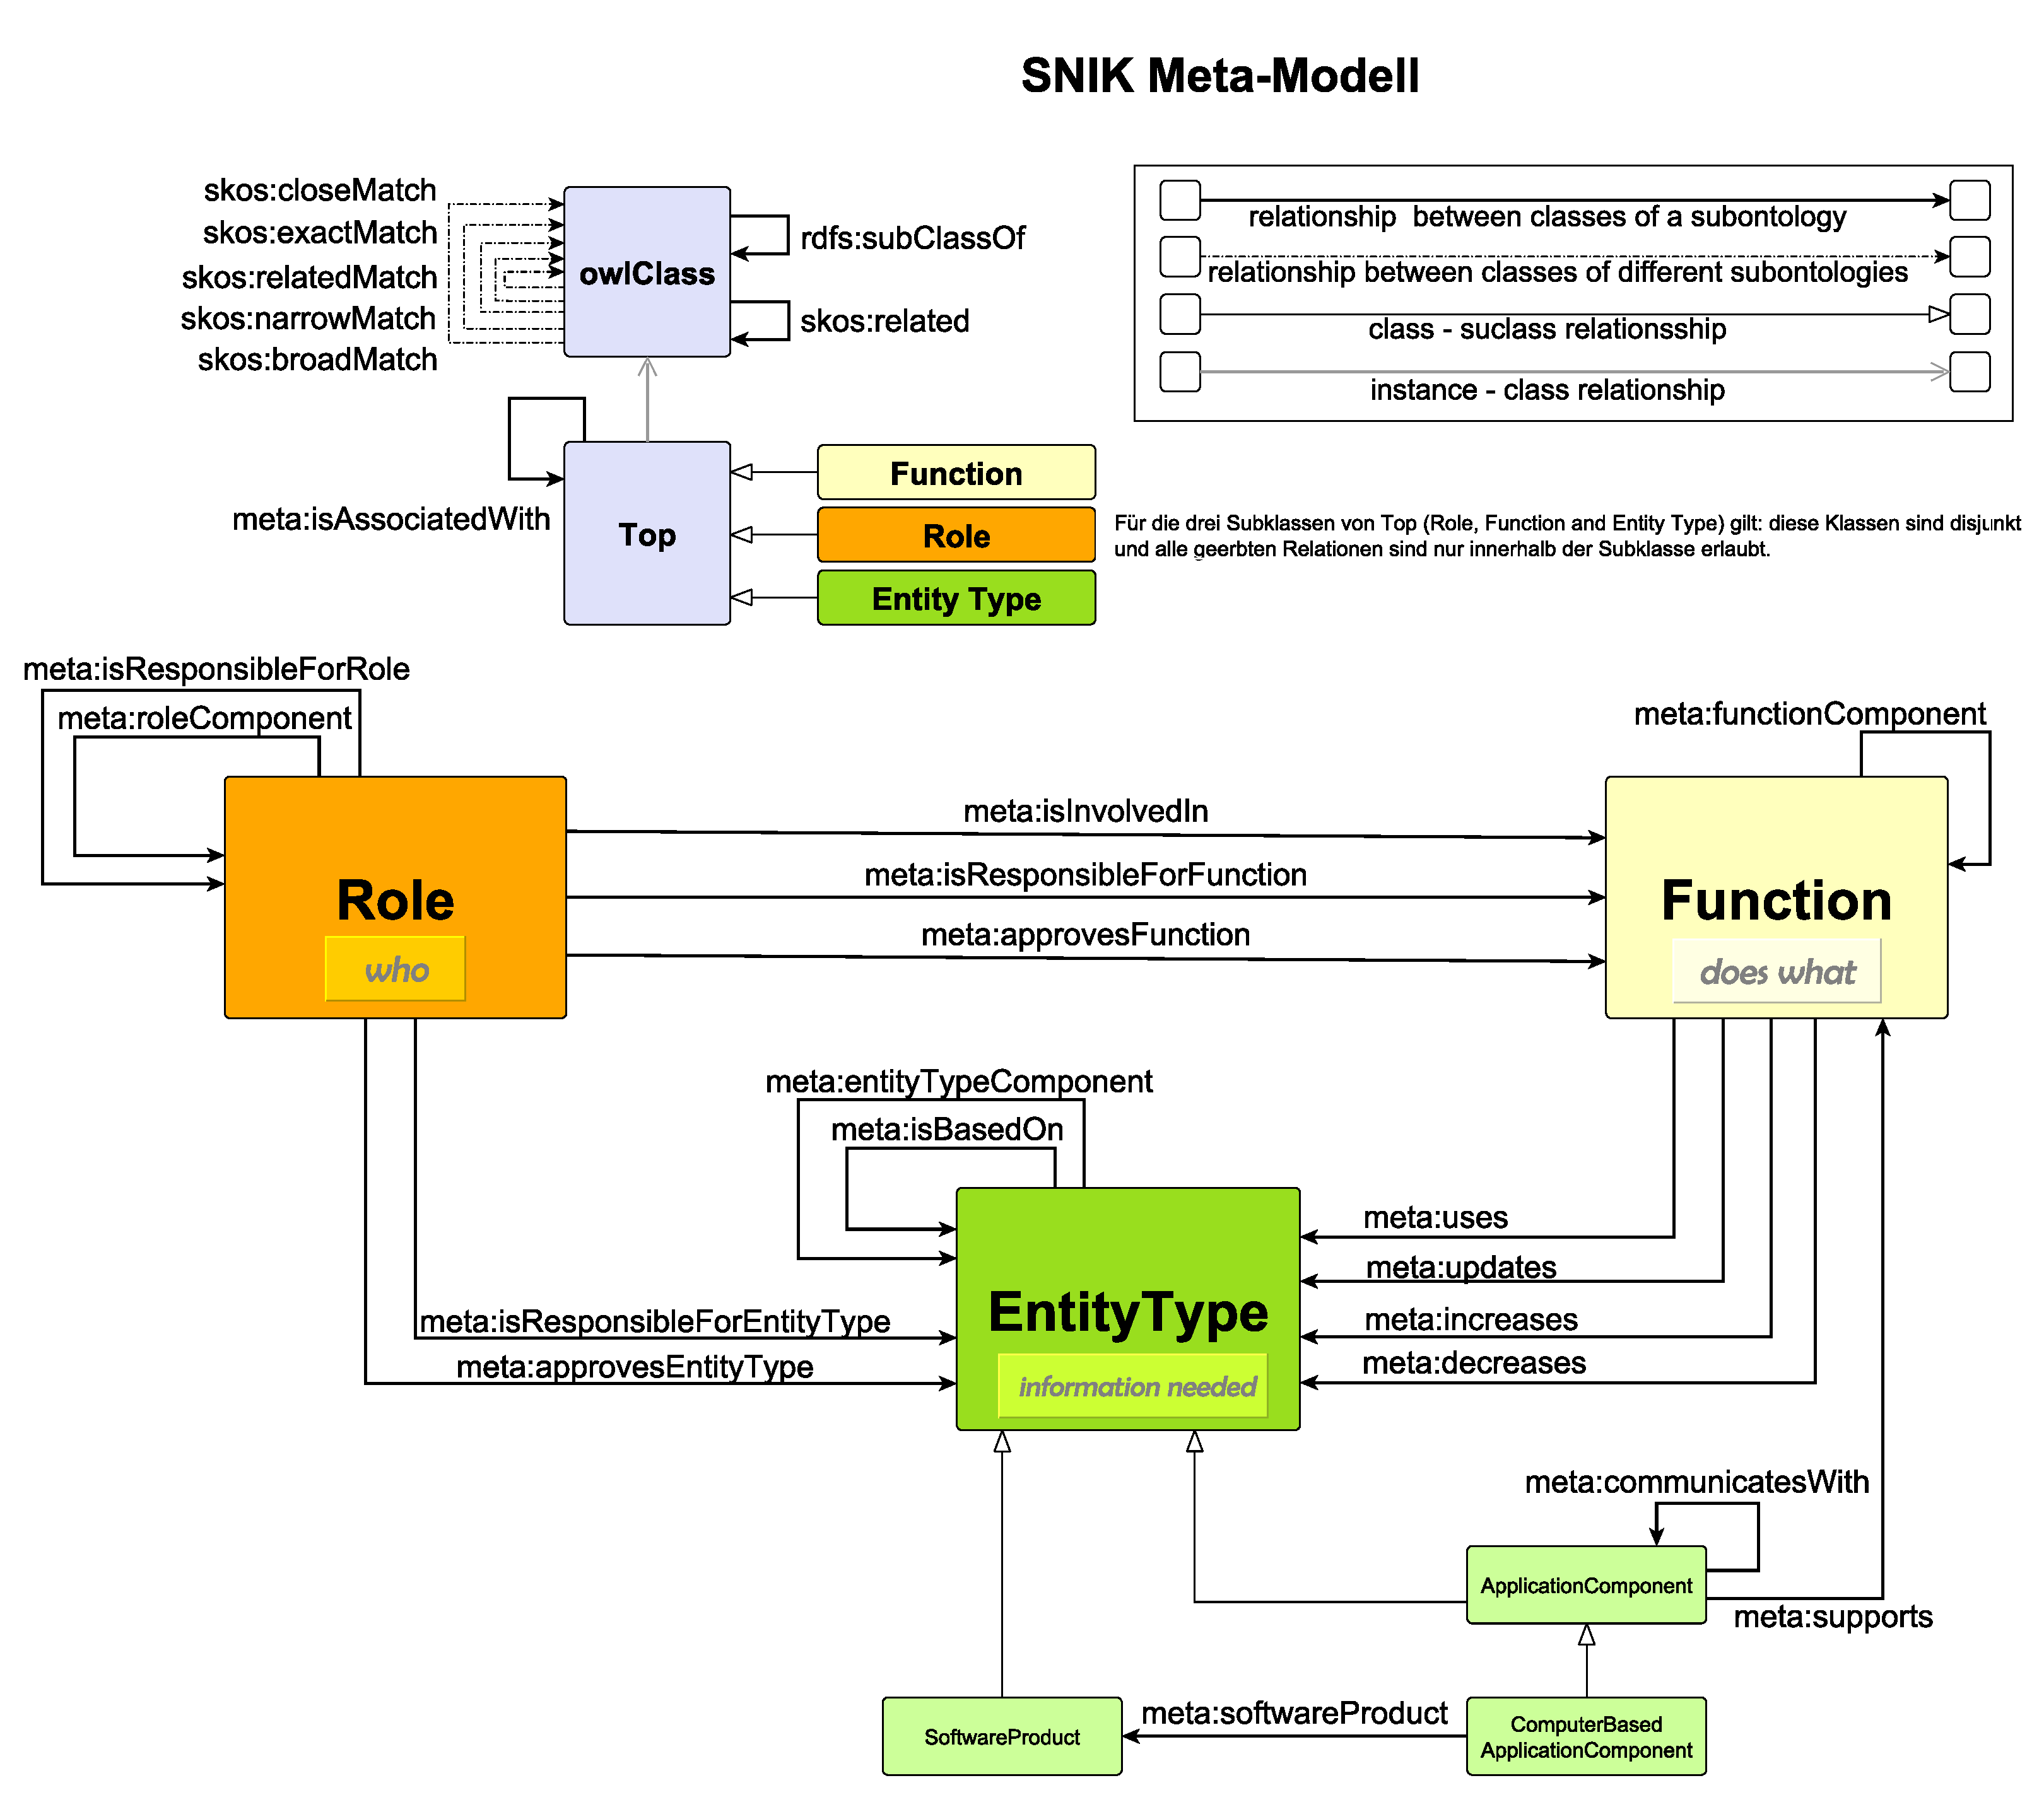
\includegraphics[width=\linewidth]{../Dokumentation/Images/snik-metamodel.pdf}

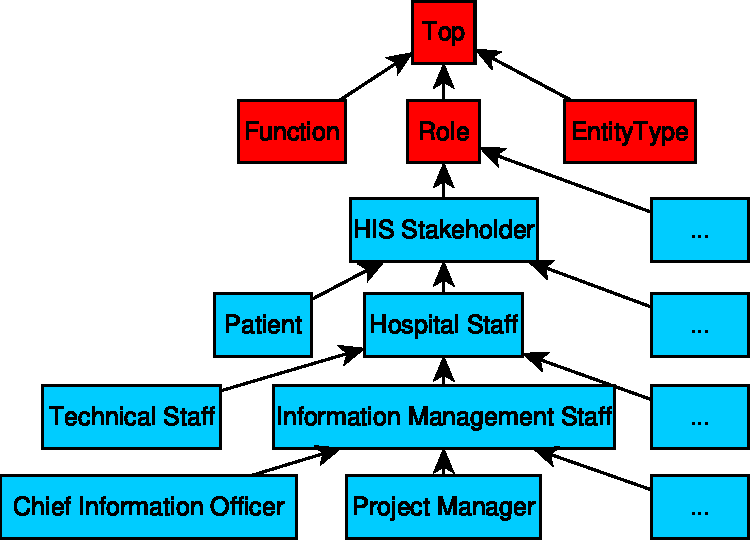
\includegraphics[width=0.5\linewidth]{../Dokumentation/Images/hierarchy.pdf}

\blindtext
\end{posterbox}
%%%%%%%%%%%%%%%%%%%%%%%%%%%%%%%%%%%%%%%%%%%%%%%%%%%%%%%%%%%%%%%%%%%%%%%%%%%%%%
\begin{posterbox}[name=methods,below=background]{Methodik}
\blindtext
\end{posterbox}
%%%%%%%%%%%%%%%%%%%%%%%%%%%%%%%%%%%%%%%%%%%%%%%%%%%%%%%%%%%%%%%%%%%%%%%%%%%%%%
\begin{posterbox}[name=results,column=1]{Ergebnisse}
\Blindtext
\end{posterbox}
%%%%%%%%%%%%%%%%%%%%%%%%%%%%%%%%%%%%%%%%%%%%%%%%%%%%%%%%%%%%%%%%%%%%%%%%%%%%%%
\begin{posterbox}[name=discussion,column=1,below=results]{Diskussion}
\blindtext
\end{posterbox}
%%%%%%%%%%%%%%%%%%%%%%%%%%%%%%%%%%%%%%%%%%%%%%%%%%%%%%%%%%%%%%%%%%%%%%%%%%%%%%
\begin{posterbox}[name=references,column=0,below=methods]{Literatur}
    \small
    \begingroup
    \renewcommand{\section}[2]{}%suppress heading
    % using bibtex ***********
    %\bibliographystyle{abbrv}
    %\bibliography{poster}
    % using biblatex *********
    \printbibliography
    %*************************
    \endgroup
    \vspace{0.3em}
    %Myproject is supported under the DFG grant numbers 1234/5-6 and 6543/2-1.
  \end{posterbox}
%%%%%%%%%%%%%%% IMISE Logo
\node [anchor=south east, inner sep=1pt,xshift=-3em,yshift=1em] at (current page.south east)
{
\includegraphics[height=1.5cm]{img/logos/imise-logo.pdf}};
%%%%%%%%%%%%%%% Medical Faculty Logo
\node [anchor=south east, inner sep=1pt,xshift=-19.5em,yshift=-1.5em] at (current page.south east)
{
\includegraphics[height=3.3cm,decodearray=0 0 0 0 0 1]{img/logos/medfak.pdf}};
%%%%%%%%%%%%%%%%%%%%%%%%%%%%%%%%%%%%%%%%%%%%%%%%%%%%%%%%%%%%%%%%%%%%%%%%%%%%%%
\end{poster}
\end{document}

